\documentclass{cours}
\usepackage{nicematrix}
\title{Sur la Stabilité Interlangue des Catégories Morphosyntaxiques\\[2pt]\small Rapport de Stage de L3}
\author{Matthieu Boyer}
\date{2024}

\begin{document}
\titlepage % Output the title page
	{}
        {\centering %
		{\Huge Sur la Stabilité Interlangue des Catégories Morphosyntaxiques\par}
                \vspace{16pt}
                {\Large Rapport de Stage de L3\par}
                \vspace{24pt}
                {\huge Matthieu \textsc{Boyer}\par}}
	{../logo_lattice}
	{\centering %
                {\huge\sc Laboratoire Lattice \par}
                \vspace{16pt}
                {\large \sc CNRS --- ENS-PSL --- Université Sorbonne Nouvelle\par}
                \vspace{24pt}
		{\Large Sous la direction de Mathieu \textsc{Dehouck}\par}}

\tableofcontents

\begin{abstract}
Dans ce rapport, nous nous intéressons à la stabilité interlangue des catégories morphosyntaxiques.
Nous avons quantifié la manière dont différentes catégories descriptives d'un langage ont différentes significations dans différents langages, et particulièrement la manière dont un concept est matérialisé dans différents langages.
Nous nous sommes tout particulièrement intéressés à la notion de cas grammatical, aux différences entre cas et à la définition fondamentale d'un cas. Nous avons également étudié la représentation des adpositions en parallèle à la notion de cas.
\end{abstract}


\section{Introduction}\label{sec:introduction}
\subsection{Contextualisation}\label{subsec:contextualisation}
\begin{quote}
	There is a fundamental distinction between language-particular categories of languages (which descriptive linguists must describe by descriptive categories of their descriptions) and comparative concepts (which comparative linguists may use to compare languages).
	{\flushright \textit{Martin Haspelmath} \cite{Has18}}
\end{quote}

Selon Haspelmath, il est possible que la manière de décrire les langues en linguistique soit basée sur des envies de comparaison, parfois mal placées.
Dans ce rapport, nous allons donc nous intéresser à la notion fondamentale de catégorie morphosyntaxique, et comparer les descriptions dans différents langages de catégories linguistiques comparatives.
Ceci permettrait de justifier la transposition de résultats d'une langue vers une autre.

\subsection{Définitions Linguistiques}\label{subsec:linguistique}
En linguistique, la morphologie est l'étude des mots, de la manière dont ils sont formés et des relations entre eux au sein dans langage.
La syntaxe est l'étude de la manière dont se combinent les morphèmes (plus petites unités de son faisant sens dans un langage) et les mots pour former des structures plus grandes comme des phrases.
La sémantique, enfin, est l'étude du sens linguistique, de comment les mots ont du sens, et de la manière dont le sens de parties d'une phrase influent sur le sens de celle-ci.\\
\medskip
La morphosyntaxe est la combinaison des aspects morphologiques et syntaxiques du langage, et examinent notamment comment les formes des mots et structures grammaticales intéragissent pour transmettre du sens dans une phrase.
Une catégorie morphosyntaxique est une propriété syntaxique, c'est à dire ayant des influences sur la structure grammaticale de la phrase, qui est marquée morphologiquement sur certains mots.
En français par exemple, le pluriel est une catégorie morphosyntaxique: il est marqué à la fin des mots et donne des informations sur quel groupe gouverne un autre groupe.
Il existe également des catégories morphosémantiques, qui ne donnent que des informations sur la signification d'une phrase et pas sur sa structure.\\
\medskip
Les cas grammaticaux sont des exemples de catégories morphosyntaxiques et morphosémantiques.

\subsection{Données et \emph{Universal Dependencies}}\label{subsec:données}
Pour étudier la thèse d'Haspelmath, nous allons considérer que les relations de dépendances (\textit{reldep}) décrites par les annotations de \textsc{Universal Dependencies} (UD, version 2 décrite dans \cite{UDv2}) sont une manière de représenter des catégories comparatives.
Une relation de dépendance est une manière de décrire les relations syntaxiques dans une phrase.
Elles se déduisent de la construction par une grammaire de dépendance ou contextuelle de la phrase.

\begin{figure}[H]
	\centering
	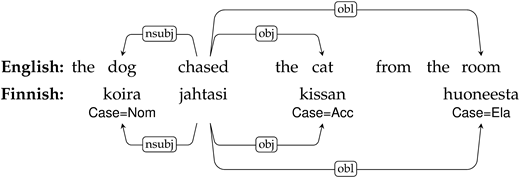
\includegraphics[width=\textwidth]{Figures/Visualisations/simplified_ud_annotation}
	\caption{Représentation d'une phrase et de ses relations de dépendances en anglais, source:\cite{UDv2}}
\end{figure}

Il existe 37 relations de dépendances de base, mais les personnes annotant les corpus ont la possibilité d'en créer de nouvelles, sous la syntaxe \texttt{str1:str2:\dots} où \texttt{str1} doit être une relation de dépendance décrite comme relation basique dans la table 3 de \cite{UDv2}.\\
Par ailleurs, les mots sont annotés avec les propriétés morphologiques qu'ils possèdent, par exemple leur temps ou leur aspect pour un verbe ou leur cas et leur genre pour un nom.
Les propriétés morphologiques universelles utilisées par UD sont décrites table 2 dans \cite{UDv2}.\\
Enfin, les mots sont annotés avec leur nature grammaticale (e.g. Nom, Verbe, Pronom\dots) comme décrits table 1 dans \cite{UDv2}.

\subsection{Méthode}\label{subsec:méthode}
Nous considérons tout d'abord que chaque \textit{reldep} décrit une unique catégorie comparative et que plusieurs \textit{reldep} ne peuvent instancier une même catégorie comparative.
En comptant le nombre d'instances de chaque \textit{reldep} pour un mot vérifiant une propriété grammaticale de la langue (i.e.\ une catégorie descriptive, que l'on représente par une \textit{feature} d'UD, typiquement les cas pour des langues en utilisant), on obtient une représentation des catégories descriptives et on peut donc mesurer la proximité de deux catégories descriptives dans deux langues différentes.
Les corpus utilisés dans cette première partie sont ceux du projet \textsc{Universal Dependencies}, version 2.14 décrite dans \cite{UD214}.

\section{Approche Géométrique}\label{sec:géométrie}
Pour cette première approche, on considère la représentation obtenue comme une représentation vectorielle: on considère qu'on se place sur $\R^{\abs{R}}$ où $R$ est l'ensemble des \textit{reldep} et dont une base est l'ensemble des relations de dépendance.
Ceci nous permet d'étudier la structure syntaxique de chaque cas d'une manière géométrique.

\subsection{Avec la distance Cosinus}\label{subsec:cosinus}
On mesure d'abord la proximité de deux vecteurs en utilisant la distance\footnote{Ce n'est pas une distance au sens mathématique} Cosinus entre ceux-ci:
\begin{equation}
	d_{\cos}(v_{1},v_{2}) = \frac{\scalar{v_{1}\mid v_{2}}}{\norm{v_{1}}\norm{v_{2}}}
\end{equation}

On obtient alors les résultats suivants pour quelques cas:

\renewcommand{\arraystretch}{1.1}
\begin{table}[H]
	\centering
	\resizebox{\textwidth}{!}{\begin{NiceTabular}{ccccccccc}
		Proximity with: & Abl & Acc & Dat & Gen & Ins & Loc & Nom & Voc \\
		First Quartile & 0.037 & 0.020 & 0.022 & 0.032 & 0.056 & 0.027 & 0.026 & 0.000 \\
		Median & 0.198 & 0.123 & 0.134 & 0.317 & 0.249 & 0.188 & 0.104 & 0.006 \\
		Third Quartile & 0.416 & 0.302 & 0.341 & 0.823 & 0.449 & 0.400 & 0.225 & 0.047 \\
		Mean & 0.259 & 0.196 & 0.214 & 0.421 & 0.282 & 0.243 & 0.159 & 0.058 \\
	\CodeAfter
		\begin{tikzpicture}
			\foreach \i in {1,...,6}
				{\draw[draw=vulm] (1|-\i) -- (10|-\i);}
			\draw[draw=vulm] (2|-1)--(2|-6);\end{tikzpicture}
	\end{NiceTabular}}
	\caption{Proximities for Case=Gen}
\end{table}

\renewcommand{\arraystretch}{1.1}
\begin{table}[H]
	\centering
	\resizebox{\textwidth}{!}{\begin{NiceTabular}{ccccccccc}
		Proximity with: & Abl & Acc & Dat & Gen & Ins & Loc & Nom & Voc \\
		First Quartile & 0.020 & 0.038 & 0.018 & 0.026 & 0.035 & 0.020 & 0.620 & 0.003 \\
		Median & 0.067 & 0.137 & 0.072 & 0.104 & 0.113 & 0.078 & 0.815 & 0.026 \\
		Third Quartile & 0.158 & 0.272 & 0.161 & 0.225 & 0.211 & 0.156 & 0.912 & 0.075 \\
		Mean & 0.115 & 0.188 & 0.119 & 0.159 & 0.153 & 0.115 & 0.739 & 0.072 \\
	\CodeAfter
		\begin{tikzpicture}
			\foreach \i in {1,...,6}
				{\draw[draw=vulm] (1|-\i) -- (10|-\i);}
			\draw[draw=vulm] (2|-1)--(2|-6);\end{tikzpicture}
	\end{NiceTabular}}
	\caption{Proximities for Case=Nom}
\end{table}

\renewcommand{\arraystretch}{1.1}
\begin{table}[H]
	\centering
	\resizebox{.9\textwidth}{!}{\begin{NiceTabular}{ccccccccc}
		Proximity with: & Abl & Acc & Dat & Gen & Ins & Loc & Nom & Voc \\
		First Quartile & 0.000 & 0.000 & 0.000 & 0.000 & 0.000 & 0.000 & 0.003 & 0.500 \\
		Median & 0.004 & 0.007 & 0.006 & 0.006 & 0.012 & 0.007 & 0.026 & 0.885 \\
		Third Quartile & 0.025 & 0.040 & 0.032 & 0.047 & 0.055 & 0.038 & 0.075 & 0.973 \\
		Mean & 0.035 & 0.042 & 0.036 & 0.058 & 0.053 & 0.042 & 0.072 & 0.681 \\
	\CodeAfter
		\begin{tikzpicture}
			\foreach \i in {1,...,6}
				{\draw[draw=vulm] (1|-\i) -- (10|-\i);}
			\draw[draw=vulm] (2|-1)--(2|-6);\end{tikzpicture}
	\end{NiceTabular}}
	\caption{Proximities for Case=Voc}
\end{table}


On observe notamment le fait que le nominatif comme le vocatif ont des directions très particulières, et sont très différents de tous les autres cas. Pour le reste, les résultats sont assez flous, et il semble difficile de tirer des résultats généraux.\\
\medskip
Par ailleurs, cette méthode est très limitée. En effet, on ne considère ici que 9 des 45 cas définis dans au moins un corpus.
De plus, les résultats donnés ici sont à pondérer par la présence de nombreux corpus/langages ne possédant pas au moins l'un des cas ci-dessus, ce qui amène à une représentation trop brouillée des informations.


\subsection{Avec l'algorithme de \textsc{Zassenhaus}}\label{subsec:zassenhaus}
On considère les espaces vectoriels engendrés par la représentation vectorielle du système de cas d'une langue, que l'on appellera \textit{espaces de cas}.
Ceux-ci sont d'une certaine dimension finie.
On applique alors sur toute paire de système de cas l'algorithme de Zassenhaus (voir \cite{zassenhaus}), permettant de générer une base de l'espace somme et de l'espace intersubsection.
Toutefois, la grande variance au niveau des coordonnées, et la trop faible dimension (au plus 45, mais souvent de l'odrdre de 5) dans un grand espace (dimension 228), rend l'intersubsection toujours nulle numériquement.
Par ailleurs, cet algorithme est très lent à exécuter car il demande de nombreux appels mémoire pour obtenir la matrice de l'espace de cas de chaque paire de cas, et demande de trouver une base de l'espace de colonne, ce qui est non-nécessairement la matrice.

\subsection{Angle entre Cas et Système de Cas}\label{subsec:projection}
On considère à nouveau la distance cosinus, mais cette fois-ci, non pas entre deux vecteurs, mais entre un vecteur et un espace de cas.
Ceci est fait en considérant le projeté orthogonal d'un vecteur sur un espace de cas et en mesurant l'angle entre les deux (ou la distance cosinus).
En observant les données de plus près, on trouve une valeur inattendue: l'angle entre le vocatif du farsi et le système de cas arabe, deux langues syntaxiquement proches, est de l'ordre de $\arccos{10^{-16}}$.
En regardant de plus près les corpus farsis\footnote{et non pas les dindes.}, on observe que cela découle d'une idiosyncracie dans les annotations.
En farsi, le lemme (unité morphologique abstraite: \textsl{fais} et \textsl{fait} sont deux graphies du même lemme \textsl{faire}, conjugué à deux personnes différentes)\label{farsi}
est décrit comme une interjection portant le vocatif et se reliant à un nom au cas absolu par la relation de transmission de cas (c'est à dire de marquer le cas pour un autre mot).
Ce lemme agit donc en réalité plus comme une adposition.
Le vocatif n'apparaît que très peu en farsi, et majoritairement dans cette situation.
Ainsi, il semble que nous ne pouvons pas tirer d'enseignements du farsi vers une autre langue, du moins sur le système de cas.
Il est toutefois bon de noter que plusieurs corpus adopte cette convention d'annotation des adpositions (cf \ref{subsec:adpos}) et certains l'adoptent également sur les adverbes.\\

\medskip
Par ailleurs, il n'est pas rare qu'au sein d'une même langue, deux corpus produisent des résultats assez différents. Ceci peut venir de la variance des phrases considérées, mais plus souvent de la présence ou non des reldeps \texttt{conj, case} et de la manière d'annoter le cas d'une adposition (cf. supra).

\subsection{Distance Euclidienne}\label{subsec:l2}
On considère cette fois la distance euclidienne entre tous deux vecteurs, qu'on aura au préalable normalisés pour qu'ils représentent des distributions de probabilité.

\renewcommand{\arraystretch}{1.1}
\begin{table}[H]
	\centering
	\resizebox{.9\textwidth}{!}{\begin{NiceTabular}{ccccccccc}
		Cas & Abl & Acc & Dat & Gen & Ins & Loc & Nom & Voc \\
		Premier Quartile & 0.605 & 0.315 & 0.552 & 0.521 & 0.535 & 0.595 & 0.569 & 0.842 \\
		Médiane & 0.781 & 0.476 & 0.725 & 0.715 & 0.695 & 0.764 & 0.722 & 0.992 \\
		Troisième Quartile & 1.002 & 0.695 & 0.950 & 0.936 & 0.929 & 0.993 & 0.965 & 1.115 \\
		Moyenne & 0.802 & 0.526 & 0.751 & 0.733 & 0.732 & 0.790 & 0.760 & 0.982 \\
	\CodeAfter
		\begin{tikzpicture}
			\foreach \i in {1,...,6}
				{\draw[draw=vulm] (1|-\i) -- (10|-\i);}
			\draw[draw=vulm] (2|-1)--(2|-6);\end{tikzpicture}
	\end{NiceTabular}}
	\caption{Proximities for Case=Acc}
\end{table}


On utilise ces données pour déterminer, entre deux corpus (ici le Czech-CLTT et le Russian-GSD), quel cas de l'autre langage est le plus proche d'un cas du premier.
Dans notre cas par exemple, le datif russe est plus proche du génitif tchèque que du datif tchèque.

\begin{table}[H]
	\centering
	\begin{tabular}{>{\tt}r|cccc}
		\toprule
		&Dat RU & Gen CZ & Gen RU & Dat CZ\\
		\midrule
		Total & 1711 & 2631 & 2070 & 277\\
		obl & 450 & 208 & 219 & 48\\
		iobj & 340 & 0 & 0 & 0\\
		amod & 243 & 736 & 475 & 54\\
		nmod & 300 & 1000 & 980 & 24\\
		conj & 112 & 225 & 84 & 21\\
		case & 0 & 340 & 1 & 87\\
		det & 34 & 80 & 79 & 3\\
		\bottomrule
	\end{tabular}
	\caption{Extraits des Vecteurs de Reldep pour le Russe et le Tchèque}
\end{table}

On enlève ensuite \texttt{conj, det} puisque ces \textit{reldep} démontrent l'accord vers la tête du groupe/de la proposition, et donc des doublons dans les données, ceci permet d'éviter de compter comme plusieurs instances d'un même cas un groupe nominal de la forme \emph{Alice, le boulanger, la laitière et Bob}, qui remplit un usage sémantique et syntaxique unique dans la phrase.
On enlève aussi \texttt{case}, qui souvent (notamment visible dans l'exemple ci-dessous), est utilisé pour marquer le cas avec une apposition (sur, sous), et ceci dépend très fortement de la personne qui a annoté le corpus, et de l'usage dans les grammaires du langage.\\
\medskip
En considérant le graphe orienté des plus proches voisins, on remarque que celui-ci ne peut pas avoir de $n$-cycle pour $n \geq 3$ et décrit des relations de proximité minimale.
Pour le tchèque et le russe, le graphe est le suivant:

\begin{figure}[H]
	\centering
	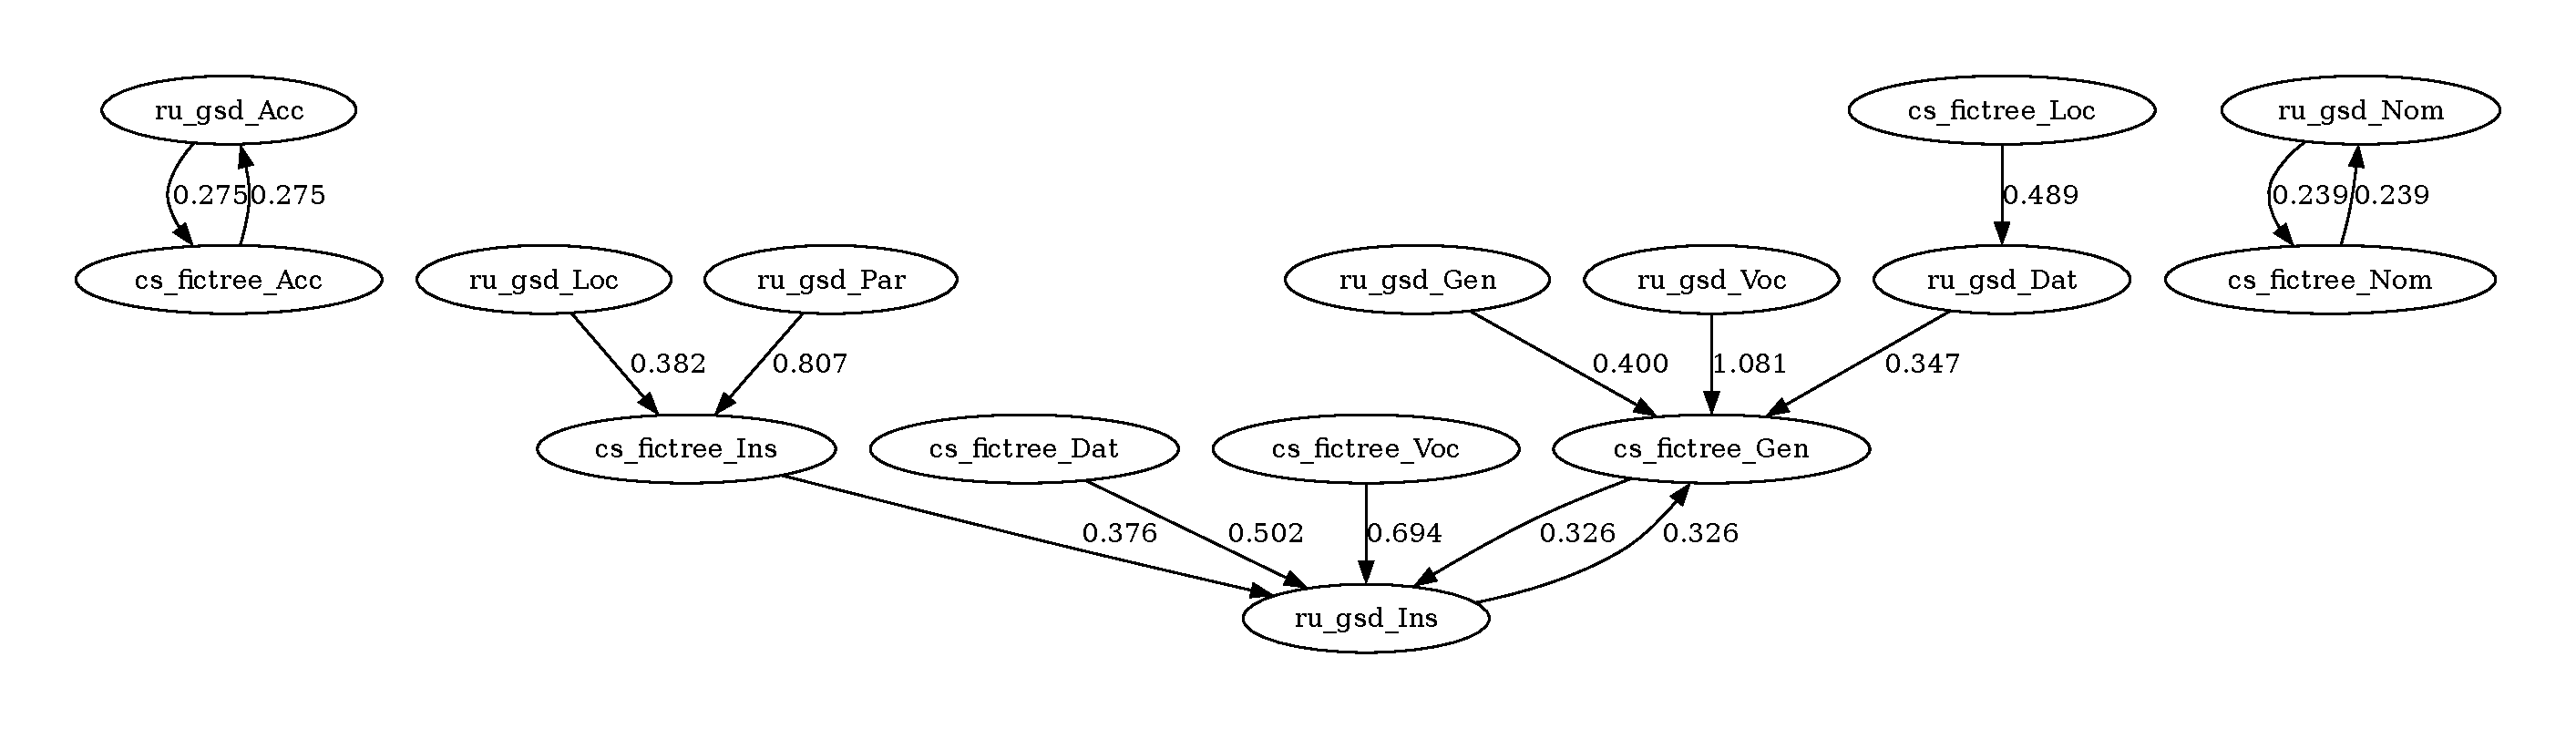
\includegraphics[width=\textwidth]{Figures/GNN/gnn_ru_gsd_cs_fictree}
	\caption{Graphes des Plus Proches Voisins Russe-Tchèque.}
\end{figure}

Pour éviter encore plus d'avoir des redites, on décide de ne se concentrer que sur des mots de même nature.
Ceci permet par exemple d'éviter qu'un groupe nominal ayant la même fonction sémantique (e.g. objet direct du verbe) apporte plusieurs instances d'un même cas (e.g. avec un adjectif et un nom à l'accusatif).
On obtient alors le graphe suivant pour le tchèque et le russe en ne considérant que les noms:

\begin{figure}[H]
	\centering
	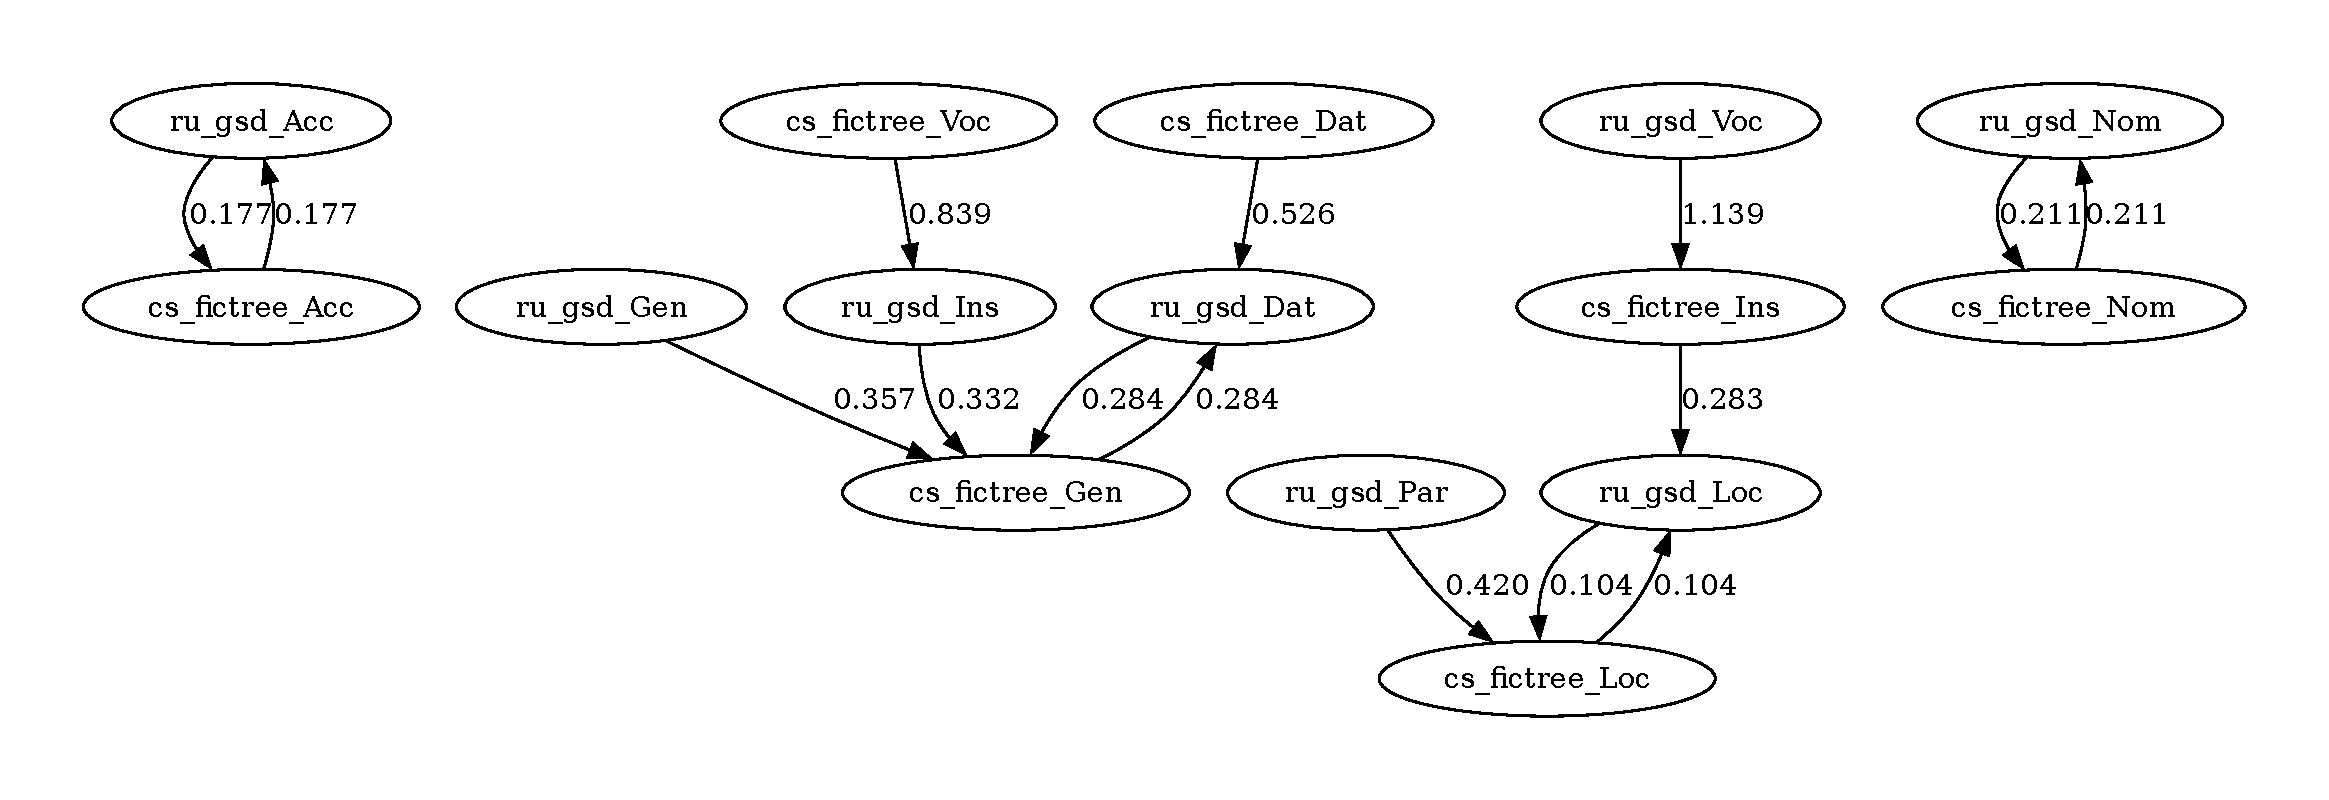
\includegraphics[width=\textwidth]{Figures/GNN/gnn_ru_gsd_cs_fictree_Nouns_Only}
	\caption{Graphes des Plus Proches Voisins Russe-Tchèque pour les Noms uniquement.}
\end{figure}

On observe notamment que pour les noms, la structure du graphe reste la même.
Le vocatif russe et le vocatif tchèque, peu utilisées et le partitif russe n'ayant pas d'équivalent en tchèque, ils sont bien plus éloignés des autres cas.
On retrouve par ailleurs un bloc datif -- génitif qui était déjà présent auparavant, à variance dans le corpus près.
Par ailleurs, on observe également que les paires accusatif -- accusatif et nominatif -- nominatif restent stables et plus proches que toutes les autres paires de cas.\\
En ne considérant que les pronoms, on obtient le graphe suivant:

\begin{figure}[H]
	\centering
	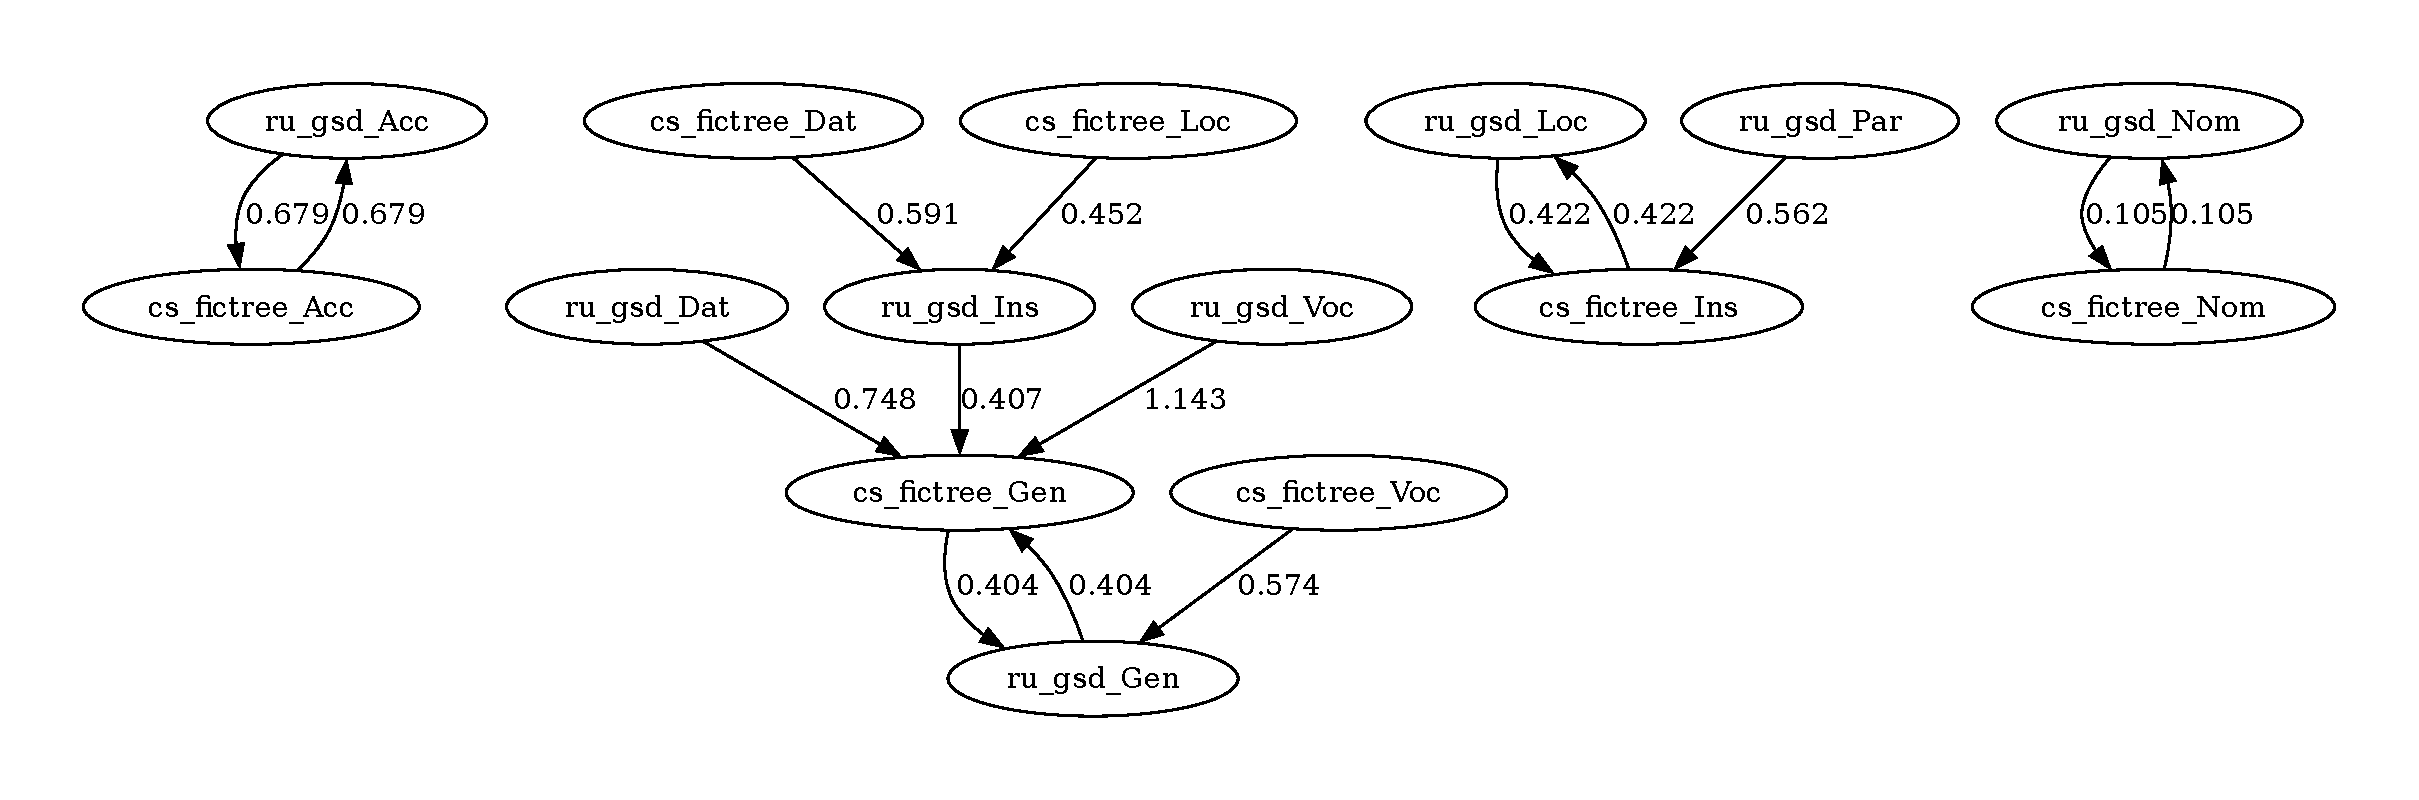
\includegraphics[width=\textwidth]{Figures/GNN/gnn_ru_gsd_cs_fictree_Pronouns_Only}
	\caption{Graphes des Plus Proches Voisins Russe-Tchèque pour les Pronoms uniquement.}
\end{figure}

Cette fois ci, il y a une variance bien plus forte dans les distances, sans doute due à la variance dans les données. En effet, à part au nominatif et à l'accusatif les échantillons de données sont bien plus faibles.

\begin{table}[H]
	\centering
	\framebox{\begin{minipage}{.45\textwidth}
	\begin{center}
	\emph{Échantillons pour les noms:}
	\medskip
	\begin{tabular}{ccc}
		\toprule
		Cas & Russe & Tchèque\\
		\midrule
		Acc & 2807 & 5960\\
		\midrule
		Dat & 1029 & 861\\
		\midrule
		Gen & 7616 & 4378\\
		\midrule
		Ins & 1642 & 2100\\
		\midrule
		Loc & 2809 & 2583\\
		\midrule
		Nom & 4571 & 5970\\
		\midrule
		Par & 1 & 0\\
		\midrule
		Voc & 1 & 203\\
		\bottomrule
	\end{tabular}
	\end{center}
	\end{minipage}}
	\framebox{
	\begin{minipage}{.45\textwidth}
	\begin{center}
	\emph{Échantillons pour les pronoms:}
	\medskip
	\begin{tabular}{ccc}
		\toprule
		Cas & Russe & Tchèque\\
		\midrule
		Acc & 206 & 5960\\
		\midrule
		Dat & 129 & 2743\\
		\midrule
		Gen & 241 & 448\\
		\midrule
		Ins & 151 & 400\\
		\midrule
		Loc & 128 & 221\\
		\midrule
		Nom & 631 & 1427\\
		\midrule
		Par & 1 & 0\\
		\midrule
		Voc & 1 & 8\\
		\bottomrule
	\end{tabular}
	\end{center}
	\end{minipage}}
	\caption{Taille d'Échantillons sur les cas en Russe et en Tchèque.}
\end{table}

Finalement, il semble que considérer les pronoms fait perdre en information car ceux-ci sont bien moins usités en général. Toutefois, on remarque également qu'une structure générale de la langue semble transparaitre de ces graphes.
Il faut cependant noter que les graphes dépendent très fortement du corpus proposé:

\begin{figure}[H]
	\centering
	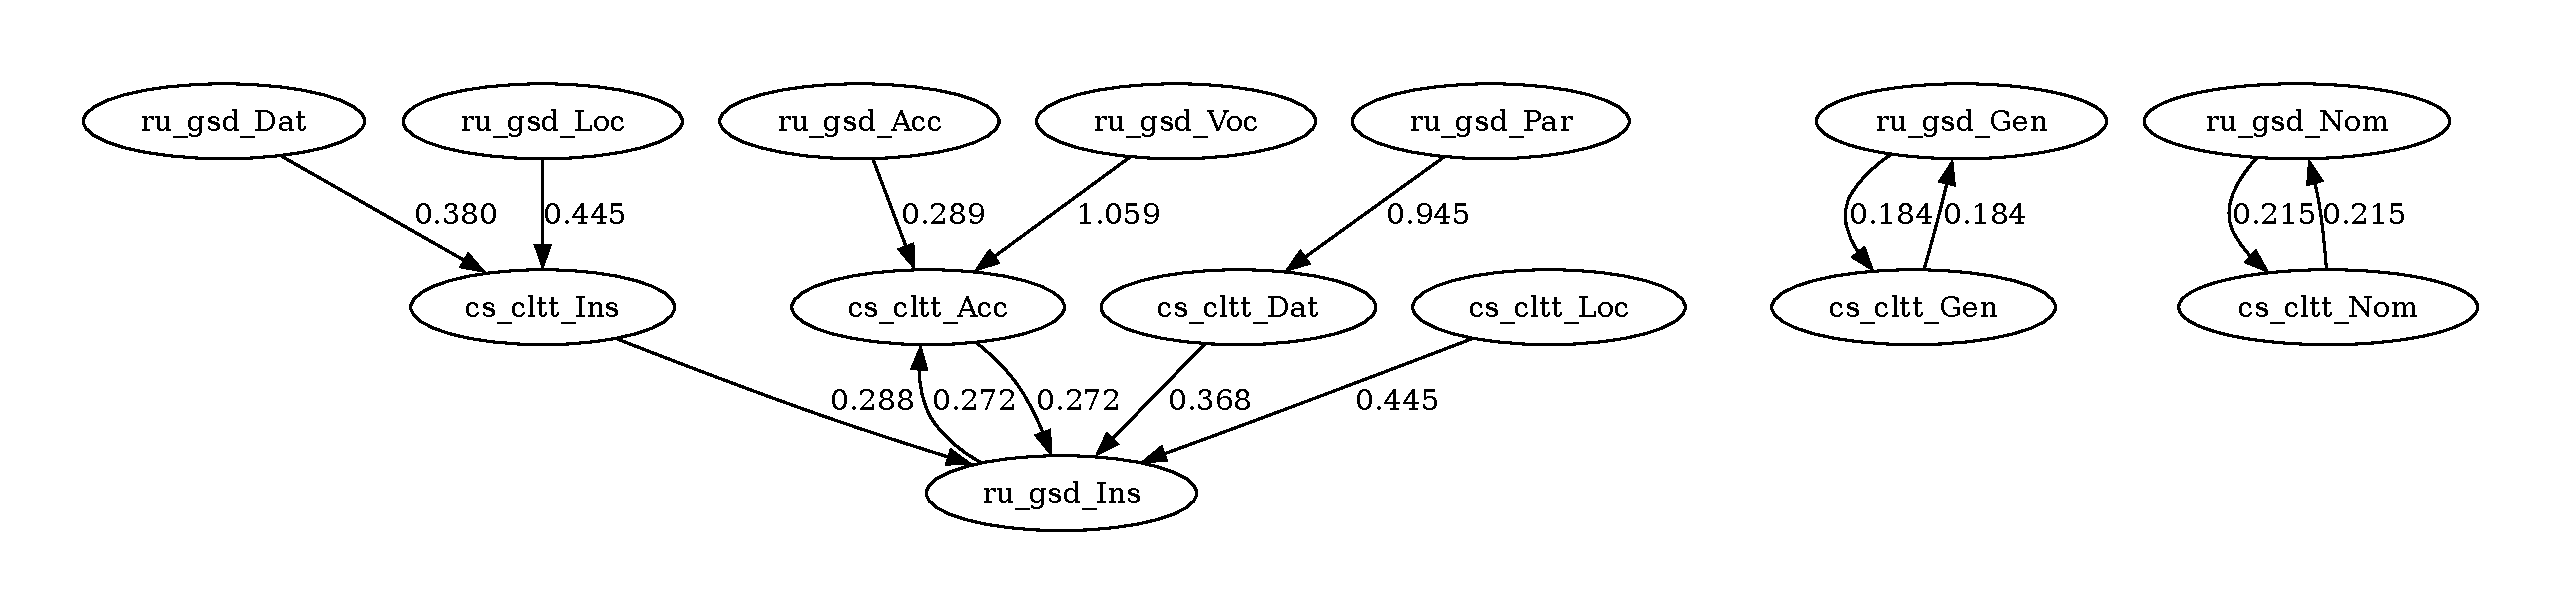
\includegraphics[width=\textwidth]{Figures/GNN/gnn_ru_gsd_cs_cltt}
	\caption{Graphe des Plus Proches Voisins Russe-Tchèque}
	\label{GNNRuCz}
\end{figure}

Ici, on ne considère plus le corpus \texttt{cs\_fictree} mais le \texttt{cs\_cltt}, bien plus petit (467 phrases contre 10160).
Même si la forme du graphe ne semble que peu changer, la variance dans le corpus joue énormément.\\
Par ailleurs, cette méthode n'est que peu applicable, puisqu'elle nécessite d'étudier toutes les langues par paire.

\subsection{Visualisation des Données}\label{subsec:vis}
Les résultats précédemment obtenus ne permettent d'observer les données ou bien à une échelle très importante, ce qui brouille les résultats, ou bien à une échelle trop faible pour qu'on puisse généraliser un résultat.
Dans la suite, on propose donc des méthodes pour regrouper les vecteurs de cas dans différentes langues, afin d'essayer de constater l'uniformité (ou non) de certains groupes de cas.

\subsubsection{PCA}\label{subsub:pca}
On commence par appliquer une analyse en deux composantes principales (PCA) aux vecteurs représentant deux cas différents.

\begin{figure}[H]
	\begin{minipage}{.5\textwidth}
	\begin{center}
	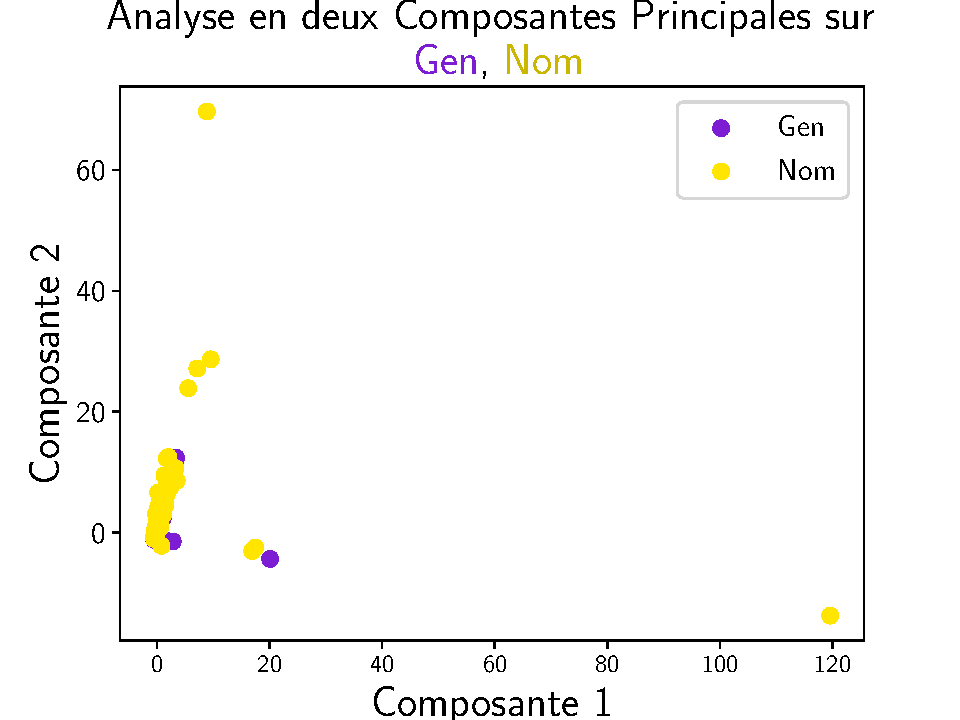
\includegraphics[width=\linewidth]{Figures/Visualisations/pca_Gen_Nom}
	\end{center}
	\end{minipage}
	\begin{minipage}{.5\textwidth}
	\begin{center}
	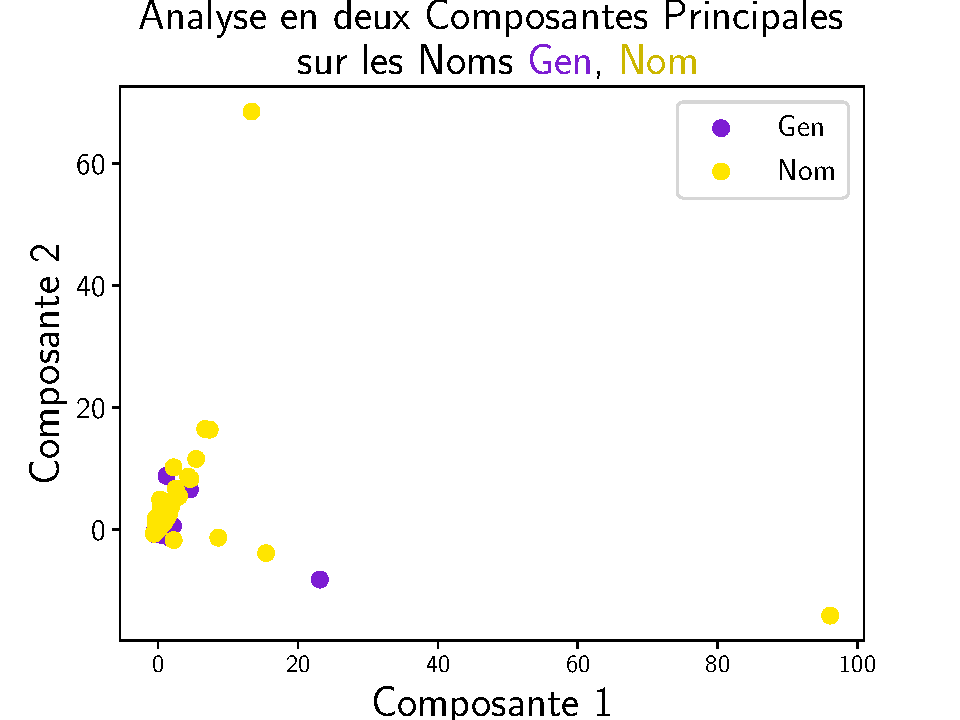
\includegraphics[width=\linewidth]{Figures/Visualisations/pca_Gen_Nom_Nouns}
	\end{center}
	\end{minipage}
	\caption{Représentations de l'Analyse en deux Composantes Principales sur le Génitif et le Nominatif}
\end{figure}

En regardant les corpus qui sont éloignés du groupe principal, on observe que les composantes déterminées par l'algorithme de PCA sont en fait basées sur deux langues, et donc les deux composantes n'ont pas de sens au regard de la syntaxe.

\subsubsection{Analyse Topologique des Données}\label{subsub:tda}
Pour l'implémentation de ce qui suit, on utilise les biblothèques Python \texttt{Gudhi}, \texttt{POT} et \texttt{Hera}, dont les implémentations sont décrites dans~\cite{Gudhi},\cite{PythonPOT},~\cite{Hera}

On utilise un complexe cubique pour essayer de représenter au mieux les groupes d'homologie (cf. \cite{tldrtda} pour les détails) de la variété triangulée par les points de chaque cas. En effet, ici, il est compliqué de calculer directement un complexe moins régulier de part le nombre de points et la dimension de l'espace.

\begin{figure}[H]
\begin{minipage}{.5\textwidth}
	\begin{center}
	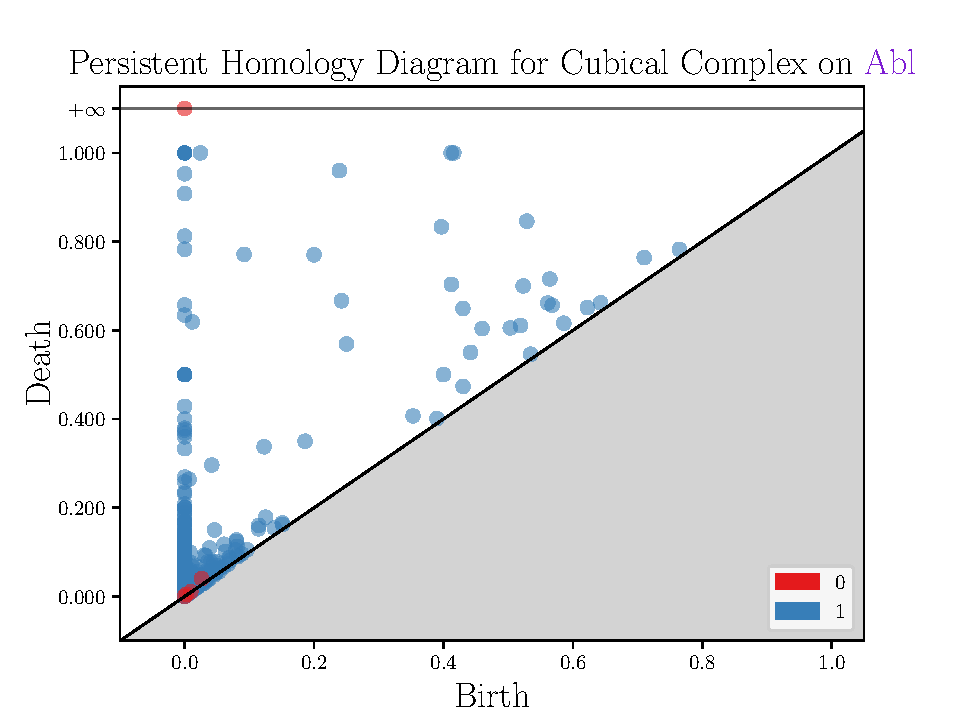
\includegraphics[width=\linewidth]{Figures/Visualisations/cc_Abl}
	\end{center}
\end{minipage}
\begin{minipage}{.5\textwidth}
	\begin{center}
	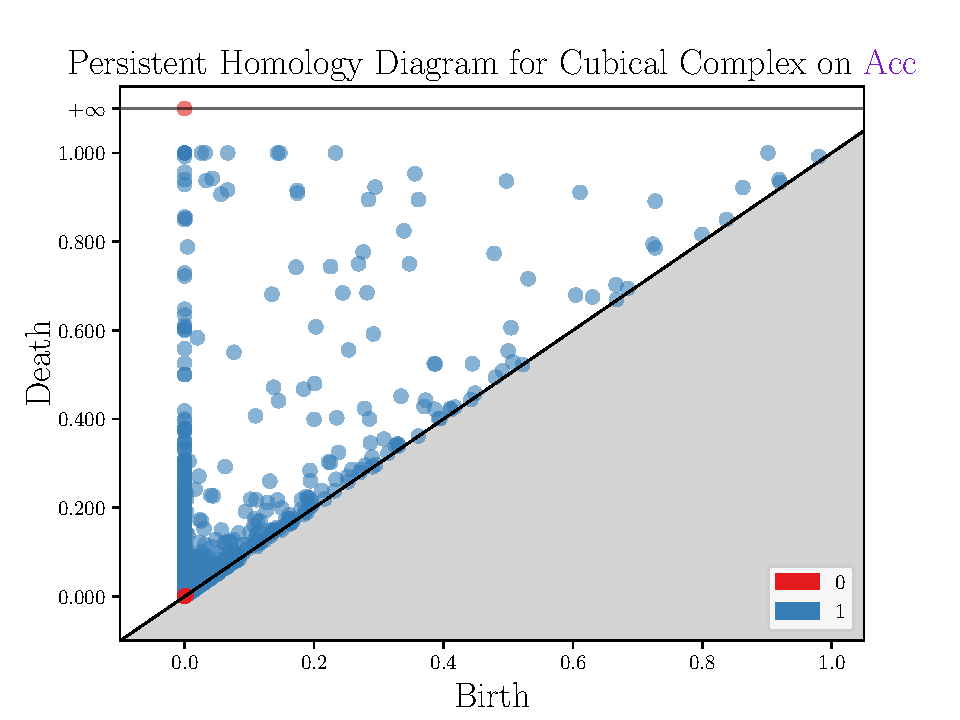
\includegraphics[width=\linewidth]{Figures/Visualisations/cc_Acc}
	\end{center}
\end{minipage}
\caption{Représentations de l'Homologie Persistente du Complexe Cubique sur $\{\tt Abl,Acc\}$}
\end{figure}

On a également calculé les complexes sur les Nominatifs et Accusatifs. On remarque qu'une forme générale se retrouve dans les diagrammes de persistences de chacun des cas.
Lorsqu'on calcule la distance de Wasserstein entre deux diagrammes, on obtient le tableau suivant:

\begin{table}[H]
\centering
\begin{tabular}{c|ccccc}
	\toprule
	Cas & Abl & Acc & Dat & Loc & Gen\\
	\midrule
	Abl & 0.00 & 2.45 & 3.11 & 1.94 & 3.85\\
	Acc & 2.45 & 0.00 & 1.33 & 1.25 & 1.79\\
	Dat & 3.11 & 1.33 & 0.00 & 1.63 & 1.27\\
	Loc & 1.94 & 1.25 & 1.63 & 0.00 & 2.26\\
	Gen & 3.85 & 1.79 & 1.27 & 2.26 & 0.00\\
	\bottomrule
\end{tabular}
\caption{Distances de Wasserstein entre les Diagrammes de Persistence des Complexes Cubiques pour quelques Cas}
\end{table}

Les distances étant assez faibles compte tenu le nombre de points (on n'a, contrairement à \ref{subsec:bary}, pas des distributions de probabilité), on obtient bien le résultat suggéré par les figures, il semble y avoir une structure générale de la notion topologique de variété engendrée par un cas.
Pour vérifier cette hypothèse, on teste de même en créant le complexe de Rips.
Toutefois, les diagrammes restant très brouillons, il est difficile de trouver une variété plus abstraite avec la même homologie.

\begin{figure}[H]
\begin{minipage}{.5\textwidth}
	\begin{center}
	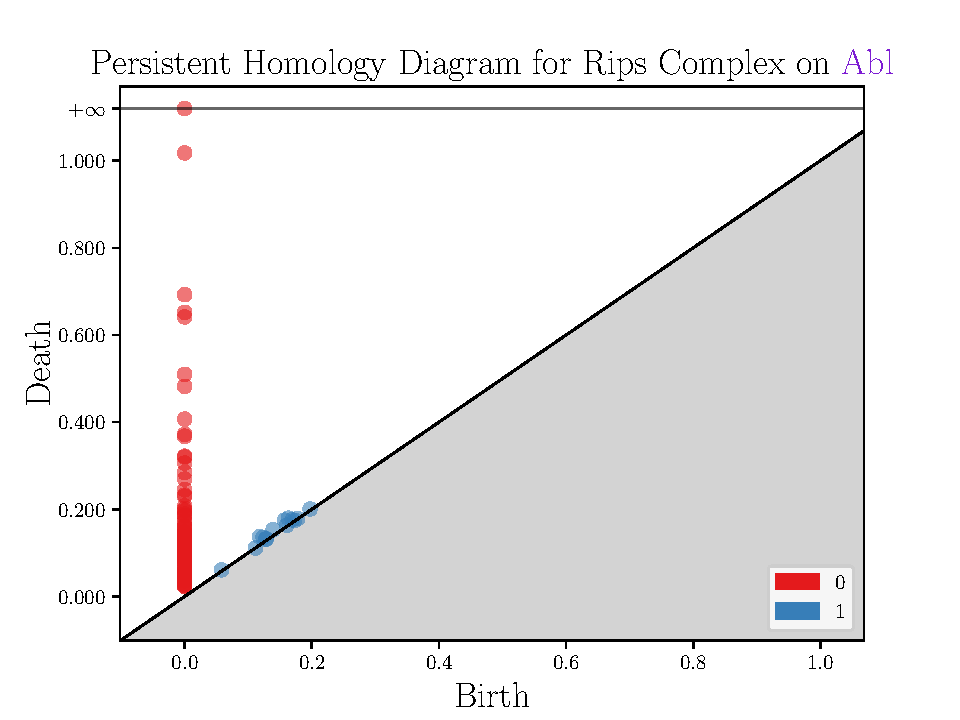
\includegraphics[width=\linewidth]{Figures/Visualisations/rc_Abl.pdf}
	\end{center}
\end{minipage}
\begin{minipage}{.5\textwidth}
	\begin{center}
	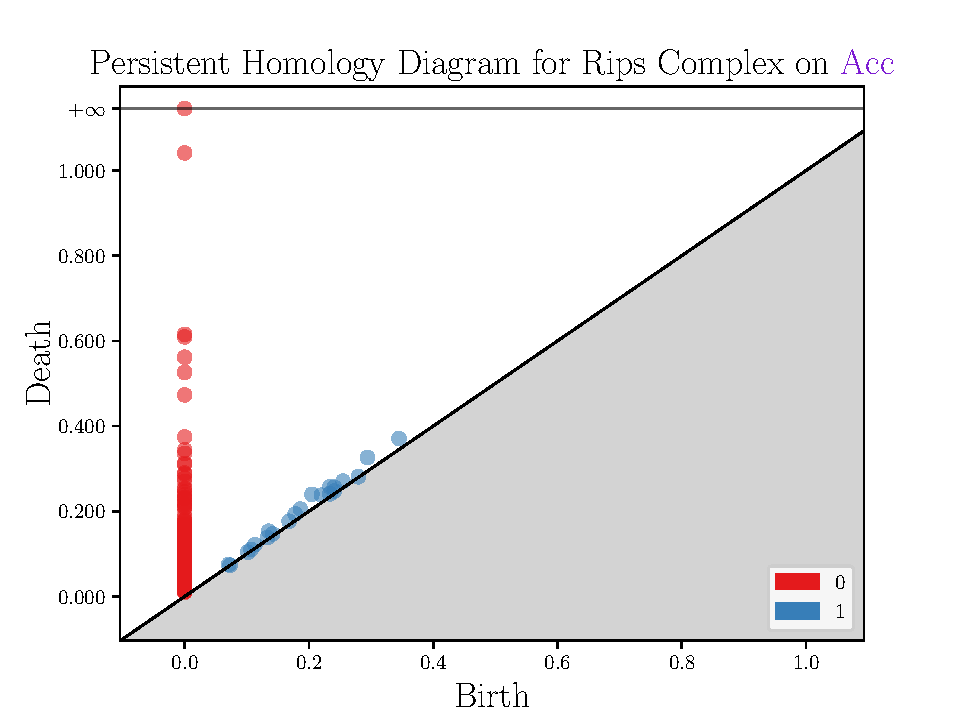
\includegraphics[width=\linewidth]{Figures/Visualisations/rc_Acc.pdf}
	\end{center}
\end{minipage}
\caption{Représentations de l'Homologie Persistente du Complexe de Rips sur $\{\tt Abl,Acc\}$}
\end{figure}

On remarque à nouveau qu'une forme générale se retrouve dans les diagrammes de persistences de chacun des cas.
Lorsqu'on calcule la distance de Wasserstein entre deux diagrammes pour quelques cas, on obtient le tableau suivant:

\begin{table}[H]
\centering
\begin{tabular}{c|cccccc}
	\toprule
	Cas & Abl & Acc & Dat & Gen & Loc & Nom\\
	\midrule
	Abl & 0.00 & 0.89 & 1.27 & 0.82 & 1.09 & 0.94\\
	Acc & 0.89 & 0.00 & 1.01 & 0.42 & 1.03 & 0.91\\
	Dat & 1.27 & 1.01 & 0.00 & 0.87 & 1.47 & 0.76\\
	Gen & 0.82 & 0.42 & 0.87 & 0.00 & 0.84 & 0.87\\
	Loc & 1.09 & 1.03 & 1.47 & 0.84 & 0.00 & 1.48\\
	Nom & 0.94 & 0.91 & 0.76 & 0.87 & 1.48 & 0.00\\
	\bottomrule
\end{tabular}
\caption{Distances de Wasserstein entre les Diagrammes de Persistence des Complexes de Rips pour quelques Cas}
\end{table}

Cela signifie notamment que la représentation d'un cas comme variété topologique ne varie que peu d'un cas à l'autre, sans toutefois pouvoir tirer plus d'informations que cela.
Intuitivement, cela signifie que si deux cas peuvent avoir des directions \textit{générales} différentes, leurs représentations seront semblables, à une rotation près.

\subsubsection{t-SNE}\label{subsub:tsne}
On essaie ensuite d'appliquer une analyse t-SNE en 2D, décrite dans~\cite{tSNE}.
Ici, on l'applique sur le Génitif et le Nominatif:
\begin{figure}[H]

\begin{center}
\begin{minipage}{.5\textwidth}
	\begin{center}
	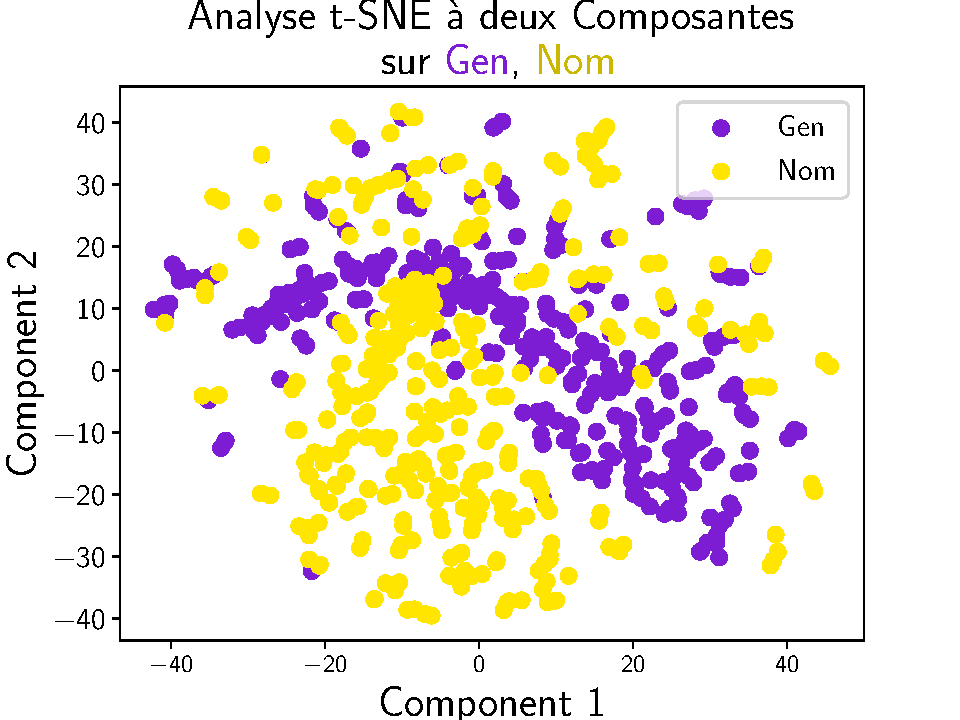
\includegraphics[width=\linewidth]{Figures/Visualisations/tsne_Gen_Nom.pdf}
	\end{center}
\end{minipage}
\end{center}

\begin{minipage}{.5\textwidth}
	\begin{center}
	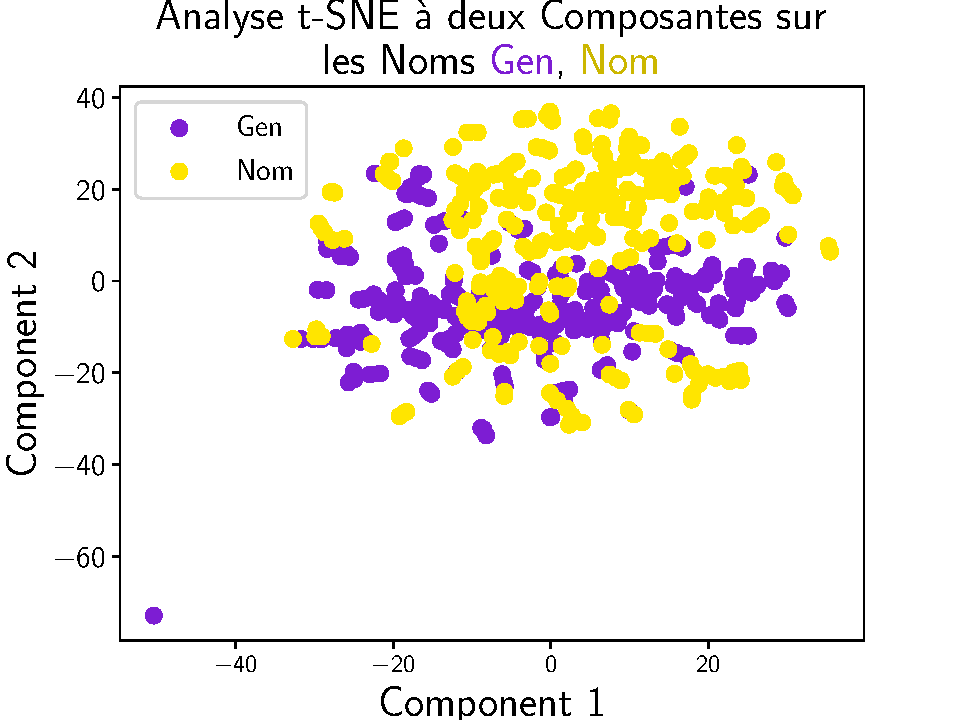
\includegraphics[width=\linewidth]{Figures/Visualisations/tsne_Gen_Nom_Nouns.pdf}
	\end{center}
\end{minipage}
\begin{minipage}{.5\textwidth}
	\begin{center}
	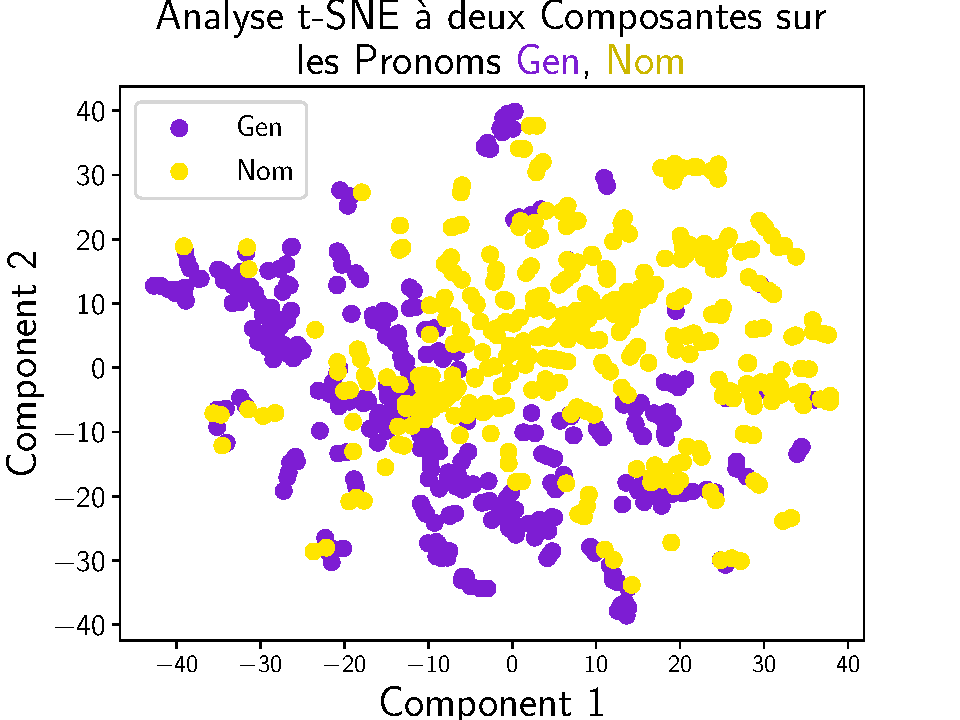
\includegraphics[width=\linewidth]{Figures/Visualisations/tsne_Gen_Nom_Pronouns.pdf}
	\end{center}
\end{minipage}
\caption{Représentations de l'Analyse t-SNE à deux Composantes sur le Génitif et le Nominatif}
\end{figure}

Il semble que deux clusters se dégagent, avec des frontières toutefois assez floues.
Il semblerait donc que syntaxiquement, le génitif et le nominatif aient des représentation assez différentes, sans toutefois savoir à quel point.

\subsubsection{Clustering avec ToMATo}\label{subsub:tomato}
On applique l'algorithme présenté dans \cite{ToMATo} avec la bibliothèque \texttt{Gudhi} (\cite{Gudhi}) sur des paires de cas, pour essayer de construire des clusters.
\begin{figure}[H]

\begin{center}
\begin{minipage}{.5\textwidth}
	\begin{center}
	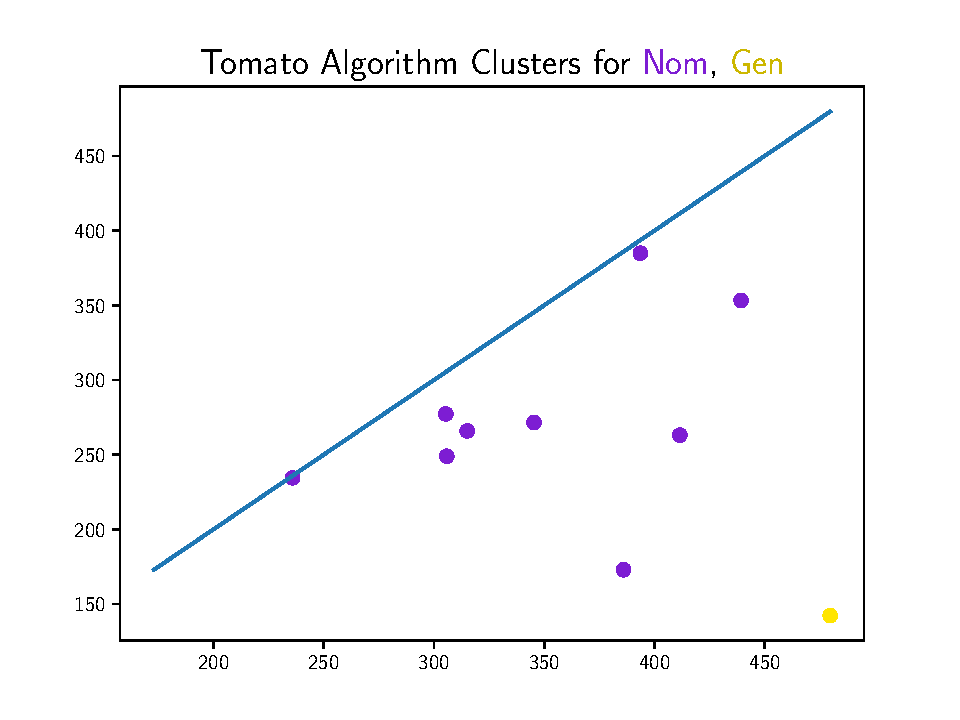
\includegraphics[width=\linewidth]{Figures/Visualisations/tomato_Nom_Gen_Nouns}
	\end{center}
\end{minipage}
\end{center}

\begin{minipage}{.5\textwidth}
	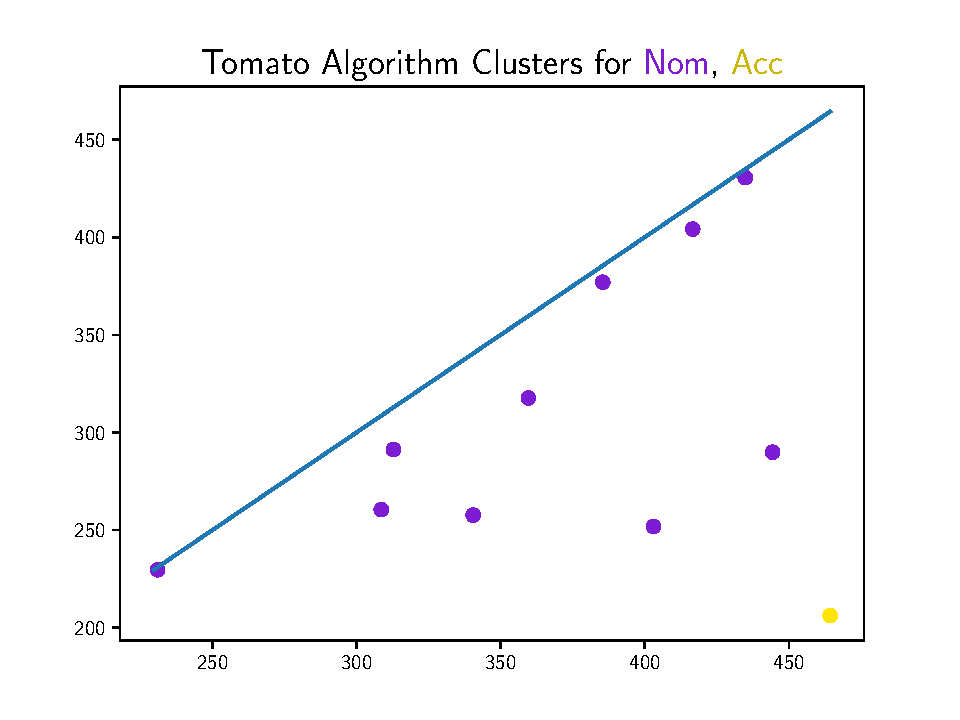
\includegraphics[width=\linewidth]{Figures/Visualisations/tomato_Nom_Acc_Nouns}
\end{minipage}
\begin{minipage}{.5\textwidth}
	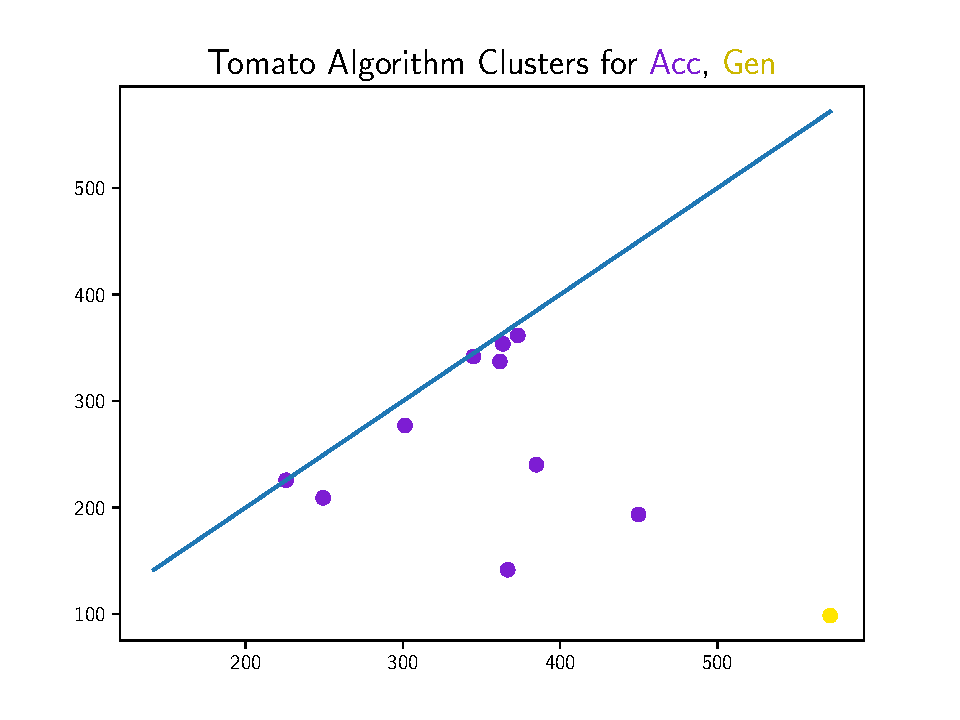
\includegraphics[width=\linewidth]{Figures/Visualisations/tomato_Acc_Gen_Nouns}
\end{minipage}

\caption{Représentations des clusters trouvés par l'algorithme ToMATo sur les paires de $\{\tt Acc,Nom,Gen\}$}
\end{figure}

Ici cependant, aucun des cas n'est clairement regroupé au sein de certains clusters, et l'algorithme ne produit aucun résultat utilisable.


\subsubsection{Clustering avec KNN}\label{subsub:knn}
Pour vérifier l'intuition qui apparaît avec le clustering proposé par l'algorithme t-SNE, on essaie d'appliquer à des listes de cas l'algorithme KNN.
On obtient la matrice de confusion suivante en appliquant l'algorithme pour $k = 11$ aux noms qui sont à l'Accusatif, au Génitif, au Locatif ou au Nominatif:
\begin{table}[H]
	\centering
	\begin{tabular}{ccccc}
		Case & Acc & Gen & Loc & Nom\\
		\midrule
		Acc & 130.000 & 62.000 & 51.000 & 34.000\\
		Gen & 69.000 & 156.000 & 16.000 & 42.000\\
		Loc & 35.000 & 57.000 & 29.000 & 34.000\\
		Nom & 29.000 & 28.000 & 9.000 & 227.000\\
	\end{tabular}
	\caption{KNN Confusion Matrix for $k = 11$ on \texttt{Acc, Gen, Loc, Nom}}
\end{table}

On observe notamment que le \emph{Locatif} est plus difficile à reconnaître que les autres cas. Ceci peut venir du faible nombre de langues possédant un locatif en comparaison aux trois autres cas.

\newpage
\section{Approche Probabiliste}\label{sec:probas}
On considère désormais qu'à un cas donné on associe une variable aléatoire $C$ sur les distributions syntaxiques dont on connaît certaines réalisations (les représentations du cas dans les différents corpus.

\subsection{Barycentrisation}\label{subsec:bary}
On a cherché jusque-là à comparer les cas.
On va désormais essayer de les prototyper et de mesurer l'écart au prototype, afin de tirer une définition des cas.
Celle-ci devrait coller à la description théorique proposée ci-dessous:
\begin{multicols}{2}
	\begin{description}
		\item[Nom] \texttt{nsubj} d'un verbe
		\item[Acc] \texttt{obj} d'un verbe
		\item[Erg] \texttt{nsubj} d'un verbe sans \texttt{obj}, ou \texttt{obj} d'un verbe
		\item[Abs] \texttt{nsubj} d'un verbe avec \texttt{obj}
		\item[Gen] \texttt{nmod}
		\item[Dat] \texttt{iobj}
	\end{description}
\end{multicols}
Pour calculer les prototypes, on procède comme suit.
On peut ainsi calculer son espérance (en considérant les mesures équiprobables), mais également le barycentre de ses réalisations pour la distance-$1$ de Wasserstein (ou Earth Mover's Distance, voir \cite{PythonPOT} pour plus de détails).
On rappelle par ailleurs que le barycentre de $n$ points pour une distance $d$ est le point qui minimise l'énergie associée:

\begin{equation*}
	P = \arg\min_{x} \frac{1}{n}\sum_{i = 1}^{n} d(x, x_{i}) = \arg\min_{x} E\left(x, \left(x_{i}\right)_{i \in \onen{n}}\right)
\end{equation*}

Ceci nous donne une forme de vecteur prototypique pour la distribution des relations de dépendance du cas.
On obtient la distribution ci-dessous, en ne considérant à nouveau que les noms, pour quelques \textit{reldep}:

\begin{table}[H]
\centering
\renewcommand{\arraystretch}{1.3}
\begin{NiceTabular}{llccccc}
				\bf Cas & \bf Prototype &\tt iobj & \tt nmod & \tt nsubj & \tt obj & \tt obl\\
	\multirow[c]{2}{*}{\bf\sc Abs}  & Uniforme    & 0.001 & 0.033 & 0.272 & 0.367 & 0.224\\
									& Wasserstein & 0.000 & 0.016 & 0.286 & 0.522 & 0.112\\

	\multirow[c]{2}{*}{\bf\sc Erg}  & Uniforme    & 0.000 & 0.007 & 0.924 & 0.005 & 0.059\\
									& Wasserstein & 0.000 & 0.005 & 0.976 & 0.014 & 0.003\\

	\multirow[c]{2}{*}{\bf\sc Nom}  & Uniforme    & 0.001 & 0.080 & 0.556 & 0.074 & 0.050\\
									& Wasserstein & 0.000 & 0.049 & 0.654 & 0.093 & 0.038\\

	\multirow[c]{2}{*}{\bf\sc Acc}  & Uniforme    & 0.006 & 0.078 & 0.038 & 0.625 & 0.205\\
									& Wasserstein & 0.000 & 0.072 & 0.019 & 0.576 & 0.259\\

	\multirow[c]{2}{*}{\bf\sc Gen}  & Uniforme    & 0.009 & 0.674 & 0.039 & 0.056 & 0.149\\
									& Wasserstein & 0.000 & 0.729 & 0.031 & 0.045 & 0.179\\

	\multirow[c]{2}{*}{\bf\sc Dat}  & Uniforme    & 0.144 & 0.149 & 0.019 & 0.000 & 0.572\\
									& Wasserstein & 0.190 & 0.164 & 0.005 & 0.000 & 0.605\\

	\multirow[c]{2}{*}{\bf\sc Loc}  & Uniforme    & 0.000 & 0.166 & 0.009 & 0.017 & 0.696\\
									& Wasserstein & 0.000 & 0.188 & 0.000 & 0.000 & 0.762\\

	\multirow[c]{2}{*}{\bf\sc Ins}  & Uniforme    & 0.000 & 0.172 & 0.014 & 0.000 & 0.660\\
									& Wasserstein & 0.000 & 0.213 & 0.000 & 0.000 & 0.738\\

	\multirow[c]{2}{*}{\bf\sc Abl}  & Uniforme    & 0.000 & 0.165 & 0.013 & 0.001 & 0.700\\
									& Wasserstein & 0.000 & 0.172 & 0.000 & 0.000 & 0.785\\
	\CodeAfter
	\begin{tikzpicture}
		\draw[vulm, double] (1|-1) -- (8|-1);
		\foreach \i in {2, 4,...,20} {\draw[vulm] (1|-\i) -- (8|-\i);}
		\foreach \i in {3, 5,...,19} {\draw[yulm!60!white] (2|-\i) -- (8|-\i);}
		\draw[vulm] (2|-1) -- (2|-20);
	\end{tikzpicture}
\end{NiceTabular}
\caption{Représentation des Principales \textit{reldep} des Prototypes pour quelques Cas sur les noms}
\end{table}

On retrouve bien la représentation attendue, ce qui découle notamment de la définition \emph{théorique} des cas. \\
Il est important de noter que les vecteurs ci-dessus ne permettent pas nécessairement de différencier tous deux cas, mais seulement de différencier leurs usages syntaxiques.
Par exemple, l'Instrumental (qui marque l'outil utilisé pour une action/un objet, e.g. dans une traduction de \textsl{J'ai mangé \emph{avec} une fourchette}, on utiliserait l'instrumental pour \textsl{fourchette})
et le Locatif (qui marque le lieu d'une action, ou d'un objet, e.g. \textsl{J'ai péleriné jusqu'à Saclay} ou \textsl{J'ai couru à côté de l'école} se traduiraient avec des locatifs\footnote{certaines langues comme le finnois possèdent plusieurs \textit{locatifs} appelés inessif, élatif, illatif, adessif, ablatif, allatif\ldots Ceux-ci servent à différencier, la destination, la direction, le lieu à côté\ldots}) sont principalement des cas morphosémantiques, au sens où ils ne modifient pas la structure de la phrase mais seulement son sens.
Ainsi, il est difficile de les différencier syntaxiquement: ils agissent principalement sur un verbe en précisant son action (\texttt{obl}), mais également sur les noms en précisant leur fonction ou leur position (\texttt{nmod}).
À l'inverse, le nominatif (sujet du verbe), l'accusatif (objet du verbe), le datif (objet indirect du verbe), l'ergatif (sujet du verbe transitif) et l'absolutif (sujet du verbe intransitif et objet du verbe transitif), sont des cas plus fortement marqués syntaxiquement et sont donc plus facilement reconnaissables.\\

\medskip
Par ailleurs, l'énergie associée au prototype obtenu en prenant la moyenne des réalisations est de l'ordre de celle du barycentre pour la distance-$1$ de Wasserstein, ce qui justifie ce que l'on pouvait inférer du tableau ci-dessus, le barycentre pour la distance de Wasserstein présente un profil similaire à la moyenne des instances.
Par exemple:

\begin{figure}[H]
\centering
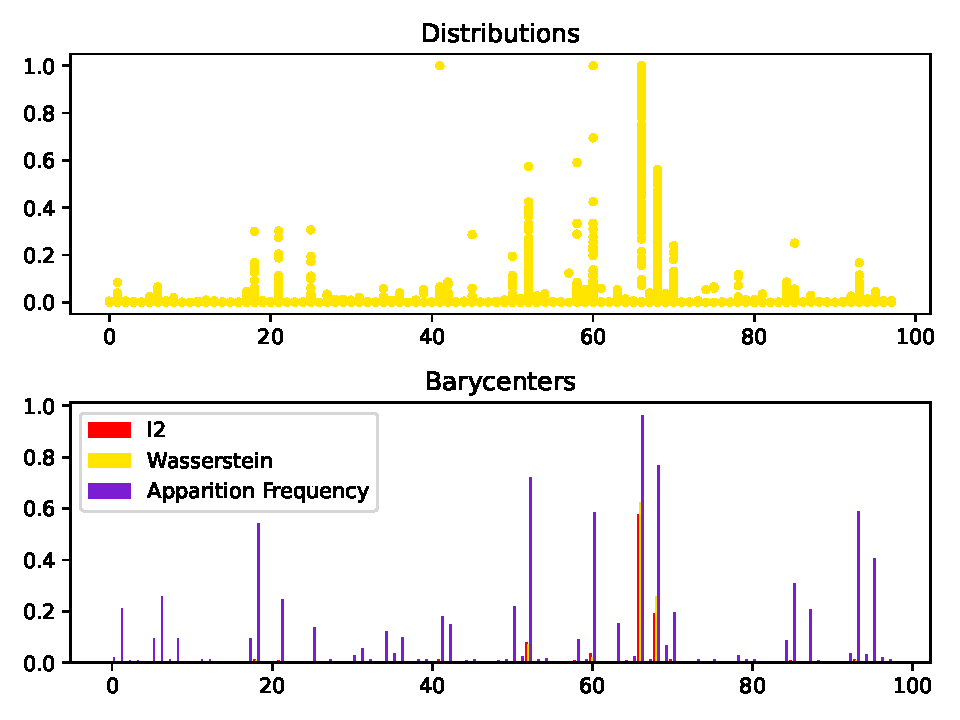
\includegraphics{Figures/Visualisations/Nouns_Wasserstein_Barycenter_Acc}
\caption{Représentation des Données et des Prototypes proposés pour les noms à l'Accusatif}
\end{figure}

Sur la figure ci-dessus, l'axe des abscisses représente les différentes \textit{reldep} apparaissant pour des noms à l'accusatif.
On représente sur le graphe du haut en jaune la fréquence associée à une reldep pour chaque corpus.
Le graphe du bas représente, en rouge, la moyenne uniforme des distributions, en jaune, le barycentre des distributions pour la distance de wasserstein, et violet la proportion des corpus pour lesquels la \textit{reldep} apparaît.
On vérifie bien notamment que pour la moyenne uniforme, certaines relations sont légèrement représentées car très présentes dans quelques langues, ce qui n'est pas le cas pour le barycentre associé à la distance de Wasserstein.


\subsection{Représentation des adpositions dans UD}\label{subsec:adpos}
Dans UD, certains corpus dénotent, lorsqu'un groupe est combiné avec une adposition (e.g. les prépositions \textsl{à, dans, par} en français, \textsl{to, into, above} en anglais, ou la postposition \textsl{ile} en turc), l'adposition comme gouvernée par la relation \texttt{case} et donnent un cas à l'adposition (cf. l'interjection farsie présentée plus haut \ref{farsi}).
Ceci découle du postulat linguistique selon lequel tous les langages humains sont également expressifs, ce qui implique qu'on peut traduire les cas par des adpositions (en français, tous exceptés le nominatif et l'accusatif).
Dans \cite{morphenglish}, Kirov, Sylak-Flassman, Knowles et Cotterell décrivent une manière d'annoter des corpus anglais selon les caractéristiques morphologiques du tchèque, langage morphologiquement riche. \\
Nous avons donc cherché à déterminer le cas de certaines adpositions.
Pour cela, on compte les relations de dépendances des cibles des relations de dépendance depuis chaque adposition.
On obtient une distribution des usages syntaxiques des adpositions, ce qui permet de comparer une adposition à un marqueur de cas.
On ne donne que la moyenne uniforme des distributions uniformes pour une même langue, le barycentre pour la distance de Wasserstein étant trop volatile pour si peu de distributions (on n'en n'a que 9 pour le français).
\begin{table}[H]
	\centering
	\renewcommand{\arraystretch}{1.3}
	\begin{NiceTabular}{>{\sc}rcccccc}
		\bf Adposition & \tt advcl &\tt iobj & \tt nmod & \tt nsubj & \tt obj & \tt obl\\
		À    & 0.01668 &  & 0.17343 & 0.00048 & 0.00381 & 0.63373\\
		Dans & 0.00466 & & 0.13780 &  & 0.00196 & 0.78694\\
		Par  & 0.00264 &  & 0.13715 & 0.00107 & 0.00178 & 0.74632\\
		Pour & 0.29543 & & 0.15867 &  & 0.00024 & 0.41168\\
		En   & 0.08128 &  & 0.17115 & & 0.00358 & 0.54076\\
		Vers & 0.00262 &  & 0.35741 & & & 0.62160\\
		Avec & 0.00613 & & 0.32369 &  &  & 0.62606\\
		De   & 0.02096 &  & 0.67966 & 0.00138 & 0.01312 & 0.14296\\
		Sans & 0.24451 & & 0.21142 & & 0.00781 & 0.43802\\
		Sous & 0.00217 & & 0.22898 & 0.00020 & 0.72797 & \\
		Sur  & 0.00477 & & 0.36267 &  & 0.00096 & 0.59385\\
		Sauf & 0.10714 & & 0.22619 & & & 0.38095\\
	\CodeAfter
	\begin{tikzpicture}
		\foreach \i in {2,...,13} {\draw[vulm] (1|-\i) --  (8|-\i);}
	\end{tikzpicture}
	\end{NiceTabular}
	\caption{Représentation de quelques adpositions en français}
	\label{tab:adpos_fr}
\end{table}
Ici, on retrouve le fait que les prépositions françaises s'utilisent dans des constructions similaires, et ne se différencient presque que sémantiquement.
Plus spécifiquement, il semble que \textsl{de} ait un caractère semblable au géniitif et que \textsl{à, dans, par, en, vers, avec, sans, sous, sur} ont plutôt un caractère semblable à l'ablatif, au locatif et autres cas syntaxiquement similaires.
Les prépositions \textsl{sauf} et \textsl{pour} quant à elle ont des usages plus particuliers, puisqu'elles servent souvent à introduire des clauses adverbiales (e.g. \textsl{il mange \ul{\emph{pour} vivre}}).

\section{Conclusion}
Nous avons pu montrer que si les cas ont une structure syntaxique générale assez similaire, il existe plusieurs familles assez distinctes au sein desquelles les cas ne diffèrent que sémantiquement.
Par ailleurs, il faut noter que le formalisme de \textsc{Universal Dependencies} et la différence dans les annotateurs cause de fortes disparités dans les manières d'annoter, notamment sur l'annotation de cas sur les adverbes et les adpositions.
Toutefois, il n'est pas illogique d'annoter un cas sur les adpositions, de par leurs fonctions sémantiques. Cependant, il apparaît que syntaxiquement elles ne sont que rarement distinguées.


\newpage
\appendix

\bibliography{report}
\bibliographystyle{alpha-fr}

\appendix
\listoftables
\listoffigures

\end{document}
